\chapter{Theoretical background}
\section{Data format in object detection}
In object detection, the goal is to locate and recognize objects of interest in the given image. The ground truth objects are represented by bounding boxes and categories. The bounding box is a rectangle that specifies the position of an object in the image and thus can be fully described by four parameters. When the model tries to localize the location of an object, it outputs a bounding box, category, and number between 0 and 1 called the confidence. Sometimes we can see a term score instead of confidence, but the meaning remains the same: certainty of the network regarding the particular prediction described by bounding box and category.

The four parameters used to describe a bounding box can be selected in multiple ways. This ambiguity led to disjoint notation. The most widespread are as follows.
\subsection{PASCAL VOC}
The format was introduced together with the PASCAL VOC dataset, which was the most popular dataset for object detection algorithm benchmarking in 2010. The bounding box is described by points $p_1(x,y),p_2(x,y)$ located in the top-left and bottom right corner. The coordinates range from 0 to image width/height in pixels. All the annotations are stored into single XML file \cite{Everingham2009,Padilla2021}.
\subsection{COCO}
COCO data format is represented by a single JSON file containing all bounding boxes of the dataset. The boxes are described by top-left corner point $p(x,y)$ and width and height of the box. Coordinated and boxes's dimensions are again in range 0 to image the dimensions. In MS COCO, the annotation can be accompanied by an additional information to solve the task, for instance a segmentation problem.
\subsection{YOLO}
This format was introduced together with the first YOLO architecture \cite{Redmon2015}, and this annotation style is still persistent when working with the YOLO-family neural networks.
In this format, the annotations are scattered into multiple TXT files, one for every image.
The bounding box is described similarly as in the COCO dataset, but the coordinates are normalized to be in the 0 to 1 range. The advantage of this approach is that when image dimensions are scaled, the annotations do not have to be modified \cite{Redmon2015,Padilla2021}.


\section{Metrics}
\subsection{Intersection over union (IOU) }
Intersection over union, also known as Jaccard index, is defined as follows: Let $B_{gt}$ and $B_p$ be a ground truth and predicted bounding box, the Jaccard index $J$ is calculated as
\begin{align}
    IOU = J(B_p, B_{gt}) = \frac{area(B_p \bigcap B_{gt})}{area(B_p \bigcup B_{gt})}.
    \label{eq:iou}
\end{align}
From the equation \ref{eq:iou} we can see that the the lowest value of IOU is 0. That means there is no overlap at all and the maximal value is 1, hence meaning a perfect match.
We use predefined threshold value of IOU to decide if the predicted bounding box matches the ground truth. Usually we choose this threshold to be 0.5 or above.

\begin{figure}
    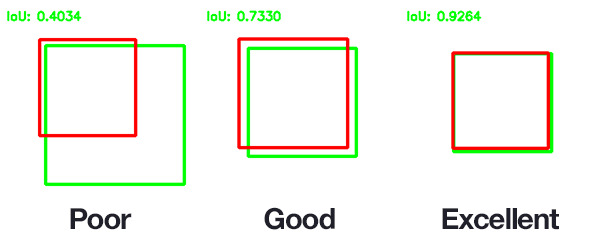
\includegraphics[width = \linewidth]{images/IOU.jpg}
    \caption{Examples of IOUs for different overlaps between GT and predicted box, source \cite{Cowton2019}}
    \label{fig:iou}
\end{figure}

\subsection{Precision and recall}
\subsubsection{Precision}
\label{subsec:precision}
When speaking about object detection, we say that a prediction is true positive (TP) if the IOU value is greater than the predefined threshold $\tau$. If otherwise, the prediction is treated as false positive (FP). Let's assume there are N predictions of our model, from which S are correct. Precision is defined as
\begin{align}
    Precision(\tau, \gamma) = \frac{\sum_{n=1}^S TP_n(\tau, \gamma)}{\sum_{n=1}^S TP_n(\tau, \gamma) + \sum_{n=1}^{N-S} FP_n(\tau, \gamma)}
\end{align}
where $\gamma$ is confidence threshold. That means we discard all predictions with confidence smaller than $\gamma$. Note that for fixed value of $\tau$ are $FP(\gamma)$ and $TP(\gamma)$ decreasing functions of $\gamma$ \cite{Padilla2021}.

\subsubsection{Recall}
\label{subsec:recall}
If there is a ground truth bounding box for which there are no given detection values of $\gamma$ and $\tau$, we say it is a false negative (FN). If we consider a dataset with G ground-truths and N predictions of which S is correct, where $(S \leq G)$, the recall can be expressed as:
\begin{align}
    Recall(\tau, \gamma) = \frac{\sum_{n=1}^S TP_n(\tau, \gamma)}{\sum_{n=1}^S TP_n(\tau, \gamma) + \sum_{n=1}^{G-S} FN_n(\tau, \gamma)}.
\end{align}
Since the value of $FN(\gamma)$ increases with the growing value of $\gamma$, we see that recall is the decreasing function of $\gamma$.
\subsubsection{F1 score}
The value of the F1 score is computed as the harmonic mean of precision and recall.
\begin{align}
    F1(\tau, \gamma) = \frac{2 \cdot Recall(\tau,\gamma) \cdot Precision(\tau, \gamma)}{Recall(\tau,\gamma) + Precision(\tau, \gamma)}
\end{align}

\subsubsection{Precision-recall curve}
From subsection \ref{subsec:precision} and \ref{subsec:recall} we were able to see that precision mostly increases as we increase the confidence threshold $\gamma$, while recall decreases. The relation between precision and recall is captured by precision recall curve. An example of precision-recall curve can be seen as the blue line in the figure \ref{fig:pr_curve}. In other words, we can say that the precision-recall curve is a mapping
\begin{align}
    \gamma \rightarrow Precision(\gamma) \times  Recall(\gamma),
    \label{eq:pr_curve}
\end{align}
where $\gamma$ ranges from 1 to 0.

\subsubsection{Mean average precision (mAP)}
To calculate MAP we first need to get the PR-curve and then interpolate the precision values. Suppose, that we have $K$ different confidence values $\gamma$ among model predictions, which are ordered as
\begin{align}
    \gamma(k),\: k = 1,2,...,K,  \; \text{such that } \gamma(i) > \gamma(j) \: for \: i > j.
\end{align}
The interpolated precision values are:
\begin{align}
    Precision_{interp}(R) = \max_{k|Recall(\gamma(k)) \geq R} \{  Precision(\gamma(k)) \}
\end{align}
The interpolated precision-recall is pictured in the figure \ref{fig:pr_curve} in red color. Now, we can compute the average precision (AP) as the area under the interpolated PR curve.
In practice, there are two different ways to approach the Reimann integral. They differ in the number of samples used to compute the integral, and are called N-point and all-point interpolation. The N-point, specifically 101 point interpolation, is used in the MS COCO competition. On the other hand, the all-point interpolation is nowadays used in PASCAL VOC challenges, after they have moved away from the 11 point interpolation.


Since the AP is calculated per class, the mean average precision is defined as the average over all categories.

In the subsections, \ref{subsec:precision} and \ref{subsec:recall}, we said that both precision and recall depend on predefined IOU threshold $\tau$ to consider prediction as true positive. This makes the value of MAP vary over different thresholds $\tau$. The threshold value used for computation of the mAP is usually denoted in the metrics name, such as $AP@.5$ in the case of MS COCO. \footnote{Note that even though they compute mean average precision, they use the $AP$ shortcut.} The standalone $AP$ without any numerical values attached to it usually refers to the official COCO metrics. The COCO metric is in its explicit form written as $AP@[.5:0.05:0.95]$ and is computed as the average of MAP values for ten different $\tau$ values, ranging from 0.5 to 0.95.

\begin{figure}
    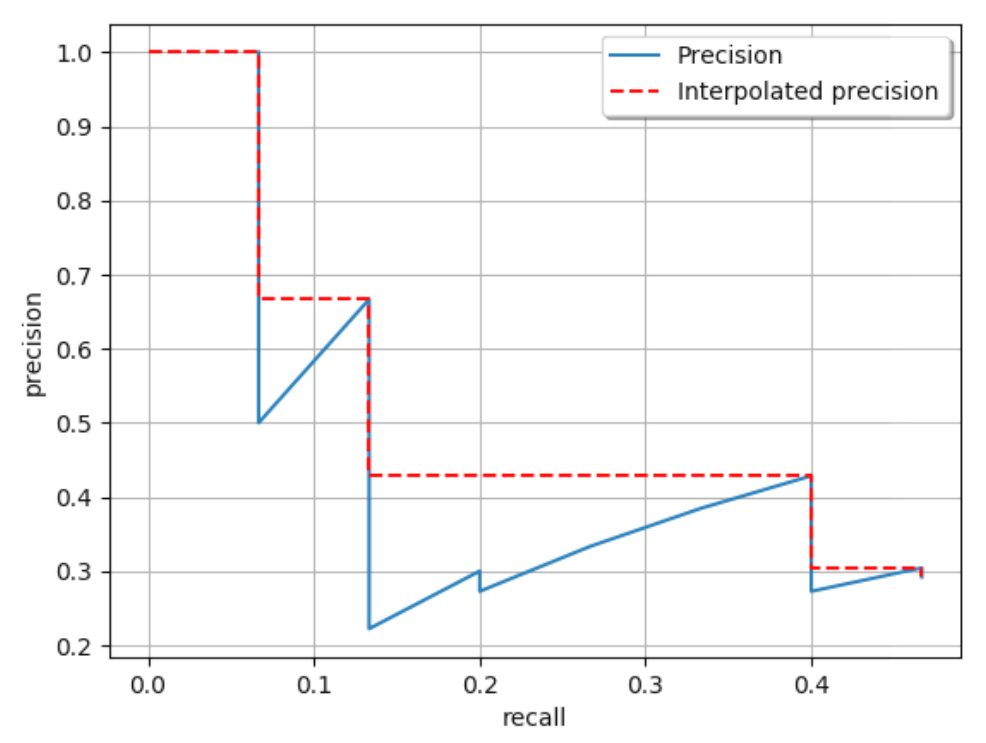
\includegraphics[width = \linewidth]{images/PR-curve.png}
    \caption{Normal and interpolated precision-recall curve, source \cite{Padilla2020}}
    \label{fig:pr_curve}
\end{figure}


\subsection{Image augmentations}


\section{Optimization}
\subsection{Learning rate schedulers}
Learning rate is considered to be one of the most, if not the most important parameter, in deep learning. It  is usually beneficial to change the learning rate during the course of training. This can be done either manually, or can be automated by an algorithm that increases or decreases the learning rate based on the set of predefined rules. This algorithm is called learning rate scheduler.

\subsubsection{Reduce learning-rate on plateau}
We couple the scheduler with a model metric and when the improvement of the metric stalls for predefined period of time, the learning rate is decreased.
The scheduler is not heavily reliant on the setting of it's hyper-parameters, making it for most of the developers a go-to choice to start from.



